\documentclass[12pt]{article}

%Required packages
\usepackage[utf8]{inputenc}
\usepackage{apacite}
\usepackage{caption} 
\usepackage{setspace}
\usepackage{amsmath}
\usepackage{graphicx}
\usepackage[textwidth=160mm, textheight=210mm, hmarginratio=1:1]{geometry}


%Prerequisite statements
\DeclareCaptionLabelSeparator*{spaced}{\\[2ex]} %Declare the caption and title seperator spacing
\captionsetup[table]{,textfont=it,format=plain,justification=justified,
  singlelinecheck=false,labelsep=spaced,skip=2ex} %Setting up caption for table titles
 \captionsetup[figure]{,textfont=it,format=plain,justification=justified,
  singlelinecheck=false,labelsep=spaced,skip=2ex} %Setting up caption for figure titles
\captionsetup{labelfont={bf}} %Bold label font for tables
\onehalfspacing %Document line spacing
\pagestyle{myheadings} %Heading style
\graphicspath{ {./figures/} } %Defining image path

\begin{document}

%Title page 
\begin{titlepage}
\begin{center}
\LARGE{\textbf{The Realtime Assessment of Mental Workload by Means of Multiple Bio-Signals}}\\
\vspace*{2\baselineskip}
\Large{\textbf{Master thesis Report}}\\
Methodology and Statistics for the Behavioral, Biomedical and Social Sciences\\
\vspace*{1\baselineskip}
Utrecht University\\
\vspace*{4\baselineskip}
{Bart-Jan Boverhof, 6000142}\\
\vspace*{1\baselineskip}
{\textbf{Thesis Supervisor}}\\
Prof.dr.ir. B.P. Veldkamp\\
\vspace*{1\baselineskip}
{\textbf{Date}}\\
October 14, 2020\\
\vspace*{1\baselineskip}
\end{center}
\end{titlepage}

%Introduction section
\section{Introduction} \label{Introduction}
The topic of mental workload has received widespread attention across a variety of different fields, amongst others the field of ergonomics \cite{young2015state}, human factors \cite{pretorius2007development} and neurosciences \cite{shuggi2017mental}.
A commonly utilized definition of mental workload, hereafter referred to as simply workload, is the demand placed upon humans whilst carrying out a certain task. As pointed out by de Waard (1996), such a definition is too shallow, for it defines workload solely in external sense. It is of importance to acknowledge that workload is a person-specific construct, for the amount of experienced workload ushered by a given task may differ across people \cite{de1996measurement}. Hence, when referring to workload throughout this research, workload in its person-specific sense is meant.

A commonly employed method for assessing workload is the NASA-Task Load Index (or TLX) questionnaire, operationalizing workload in clusters of six different dimensions \cite{hart2006nasa}. Such an assessment is usually conducted post experiment, which in certain situations could be unpractical. For example, consider an experiment with the objective of the assessing workload for pilots during a flight. Only well after the flight a measurement in the form of a questionnaire can occur, potentially generating bias. An example of such a bias is the observer bias, prescribing that actors participating in an experiment tend to over-exaggerate the treatment effect, i.e. the degree if perceived workload, when having to report it themselves post-experiment \cite{mahtani2018catalogue}.

An alternative method for assessing workload is the measurement of bio-signals during the experiment, with which the degree workload is being classified. Examples of such bio-signals, hereafter referred to as modalities, include techniques such as electroencephalogram, eye tracking, galvanic skin response, functional near-infrared spectroscopy, etc. The advantage of this approach is that complementary information streams, each stemming from a different modality, can all be interpreted simultaneously \cite{ramachandram2017deep}. This yields an objective and rich multifaceted classification of a mental construct, such as workload. Additionally, a separate model for each individual can be trained, catering towards the personal perception of workload for that specific individual. This approach comes however at the cost of an increase in complexity, residing in the need to construct a complex framework that inputs the data from each of the utilized modalities, and ultimately outputs a single classification outcome. 

The current research builds upon previous research conducted by \citeA{dolmans2020perceived}, who proposed a framework for multi-modular classification of workload with deep-learning. This research differs from this previous endeavor in that it utilizes different modalities and thus different data. However most importantly, the current research differs in that it investigates the feasibility of a real-time approach. Real-time in this sense considers the real-time classification of workload, that is classification whilst the experiment takes place. Doing so enables the possibility conduct a dynamic experiment, the state of which can be altered by responding towards the classified degree of workload for a participant. Consider a simulation with the objective of educating its participant, such as a flight simulator with the objective of educating trainee pilots. In such a situation, the ability to alter the state of the experiment dynamically, that is based on the amount of perceived workload, could substantially enhance the learning experience of a single session. Operations with which the trainee perceives high workload possibly require more practice, which could be dynamically integrated in the remainder of the experiment. Doing so has the potential of dramatically increasing the effectiveness of a single simulation session, hereby possibly entailing a more efficient learning process. 

In order to build both frameworks, three modalities are included. These modalities include the techniques of electroencephalogram hereafter referred to as EEG, galvanic skin response hereafter referred to as GSR and photoplethysmography hereafter referred to as PPG. It is important to stress that the objective of the current research is not to gain insight into the most optimal model design for each of these previously delineated modalities. It is rather to construct a framework with which real-time classification can be managed, and to which modalities of choice can easily be added. Consequently, one of two design principles on which the architecture of the framework reclines is the principle of modularity. Modularity refers to the extent to which different modalities can freely be added and/or removed to the framework, without the necessity to re-architect and rebuild it entirely. The second adhered design principle is the principle of generalizability, prescribing that the framework should not solely be utilizable in the context of workload, but also for the measurement of other mental constructs.

A deep-learning approach towards the construction of the real-time multi-modular framework is endeavored. Considering the complexity and sheer size of such a network, an important point of attention is speed. In order for real-time classification to be possible, a swiftly classifying and hence optimized network is requisited. The challenge in real-time classification with deep-learning is often not reaching adequate performance, but rather to attain adequate speed of classification. Deep neural networks easily constitute thousands of calculations made simultaneously, which is even more so for a multi-modular approach. In order for real-time classification to work, classification cannot take too long, for if it does it is not real-time anymore. Firstly, for each of the three modalities a single-modular network is constructed and assessed in terms of speed and performance. Secondly, a multi-modular network is architected, and also assessed in terms of speed and performance. Additionally, several variations to this multi-modular framework are considered. These variations differ in their size, e.g. the amount of neurons and filters. The objective of the current research is to explore the circumstances in which a multi-modular approach by means of deep learning is capable of real-time classification, whilst still ensuring ample performance with respect to classification accuracy. Ultimately, this line of research pursues the ability to conduct a dynamic experiment for multiple people simultaneously, of which the state can be altered in real-time. 

\section{Methods}

\subsection{Related Work} \label{Relatedwork}
The current section will provide an overview of previous research on the most optimal network architecture for each modality separately. Additionally,  the most feasible architecture for the multi-modular framework in its entirety will be explored. In particular, attention is placed upon the data fusion strategy, the real-time component and several model optimization techniques.

\subsubsection{First modality: Electroencephalogram (EEG)}
The first utilized modality is EEG, which constitutes a technique that detects electrical activity in the brain using electrodes. EEG is a widely utilized method for classifying workload. An overview of the complete literature on EEG classification with deep learning has been made by \citeA{craik2019deep}, who reported a total of 16 \% of all available papers to constitute with workload, lending credence to the ability of EEG as classifier of workload. Additionally, the usage of deep learning techniques for a range of different EEG application was investigated upon. Summarizing, it was reported that studies mostly found deep belief networks and convolutional neural networks to perform best when classifying workload, and advice one of these approaches as a consequence \cite{craik2019deep}.

Research by \citeA{schirrmeister2017deep} contrasted the performance of several convolutional neural networks, hereafter referred to as "ConvNets", against the widely acknowledged baseline method for EEG classification, filter bank common spatial pattern, hereafter referred to as "FBCSP". The investigated networks included a deep, a shallow, a deep-shallow hybrid and a residual ConvNet. Both the deep and shallow ConvNets were found to reach at least similar, and in some regard better classification results, as compared with the FBCSP baseline. Altogether, a deep ConvNet with four convolutional-max-pooling blocks was found to perform best, displaying an accuracy of 92.4 \% \cite{schirrmeister2017deep}.

A different approach is proposed by \citeA{tabar2016novel}, combining a ConvNet with a Stacked auto-encoder network, hereafter referred to as "SAE". Within this network, the input layer feeds into a convolutional layer with the objective of learning the filters and network parameters. The output of this convolutional layer subsequently feeds into SAE part of the network, constituting an input layer, 6 hidden layers and an output layer. A classification accuracy of 90 \% was acquired with this model \cite{tabar2016novel} . 

\subsubsection{Second modality: Galvanic Skin Response (GSR)}
The second utilized modality is GSR, measuring sweat gland on the hands and hereby inferring arousal. GSR activity have been found to significantly increase as a consequence of an increase in task workload, hence constituting to be an objective predictor \cite{shi2007galvanic}. 

Sun and colleagues explored the most optimal deep learning network for classifying six different emotional states by means of GSR data. Several models were investigated upon, amongst others a support vector machine, a ConvNet, a long-short-term-memory model and a hybrid model combining the ConvNet and long-short-term-memory, herefater referred to as "LSTM", approaches. The hybrid model was found to perform best, exhibiting an accuracy of 74\% \cite{sun2019hybrid}. 

A variant on the CovNet LSTM model was employed by \citeA{dolmans2020perceived}, who aimed to classify workload by means of, amongst other modalities, also GSR. The performance of this model was contrasted with a network consisting solely of fully connected dense layers. Conform with findings by  \citeA{sun2019hybrid}, the hybrid model was found to perform best, displaying an accuracy of 82 \% \cite{dolmans2020perceived}. The model architecture as utilized by \citeA{dolmans2020perceived} deployed two convolutional max-pooling blocks and two LSTM layers.

\subsubsection{Third modality: Photoplethysmography (PPG)}
The third modality constitutes PPG, which is a technique utilized to measure heart rate. PPG is, not undeservedly, a widely deployed technique within the field of workload classification. Zhang and colleagues investigated several approaches for measuring workload, comparing in total four modalities, out of which one was PPG. PPG was found to display both the highest sensitivity and reliability for measuring workload, lending credence to the feasibility of PPG as a method for classifying workload \cite{zhang2018evaluating}. 

Work by \citeA{biswas2019cornet} investigated upon a deep learning approach towards PPG classification, with the objective to perform both bio-metric identification and obtain heart rate information. Exceptional results were attained with a neural network, attaining an average accuracy of 96 \% \cite{biswas2019cornet}. This performance was managed with a hybrid model, incorporating two convolutional max-pooling blocks, followed with two LSTM layers. 

\subsubsection{Fusion strategy}  
When architecting a multi-modular network, information streams stemming from different modalities are required to be combined, i.e. "fused", at one point in the network in order to ultimately result in a single classification. Fusion can be done at different locations, and in different ways. Several fusion strategies as proposed by \citeA{ramachandram2017deep} have been considered.

Early, or data-level, fusion focuses on how to optimally combine data sources, before being fed into the network. Techniques that realize this include for example principle component analysis or factor analysis. Early fusing is usually challenging, especially for a multi-modular situation such as the current. This resides in the fact that data stemming from different modalities often differ with regards to dimensionality and sampling rate. Another disadvantage of early fusing, is that usually the oversimplified assumption of conditional independence is made. This assumption is unrealistic in practice, for data stemming from different modalities are expected to be correlated \cite{ramachandram2017deep}. 

Late, or decision level, fusion on the other hand refers to the process of aggregating the decisions from multiple models, each separately applied on each modalitiy separately. In case the data sources stemming from the various modalities are either correlated or ultimately inhibit a different dimensionality, late fusion is a much more feasible approach \cite{ramachandram2017deep}.

Lastly, intermediate fusion is the most widely employed fusion strategy for multi-modal deep learning problems. Modalities are fused by concatenation and adding a higher order layer, to which the individual networks, separately defined for each modality, feed into. This need not be a single layer, but could be multiple layers, as long as each modality ultimately feeds into the highest order output layer. The depth of the fusion (i.e. the amount of fusion layers) can be chosen conform the specific situation, posing intermediate fusion to be the most flexible, and therefore the most widely utilized fusion strategy \cite{ramachandram2017deep}.

Indeed, when consulting the literature, intermediate fusion strategies are the most prevailing for multi-modular deep neural networks. When taking such an approach, one is required to consider the design of this higher order network. \citeA{rastgoo2019automatic} utilize a multi-modular ConvNet approach, and fuse the modalities by concatenation, followed with two LTSM layers, two dense layers and a softmax layer. A simpler approach is utilized by	\citeA{han2020classification}, who utilized an intermediate fusion approach solely consisting of several fully connected dense layers, and ending with a soft-max layer. Lastly, \citeA{dolmans2020perceived} used a relatively deep intermediate fusion approach, consisting of two dense layers, two convolutional layers followed by another two dense layers.  

\subsubsection{Model optimization}
The technique of batch normalization was proposed by  \citeA{ioffe2015batch},  and is often applied in deep learning with the objective of enhancing the stability of a network. This is endeavored by including a batch normalization layer after each convolutional layer, re-centering and re-scaling the input feeding into this layer. If incorporating a batch normalization layer, it is recommended to do so before feeding into the activation function \cite{ioffe2015batch}. An increase in accuracy for EEG classification was attained by \citeA{dolmans2020perceived} and \citeA{schirrmeister2017deep} by specifying a batch normalization layer after each convolutional layer. Equally so, the best performing model for PPG data as proposed by \citeA{biswas2019cornet} included a batch normalization layer after each convolutional layer.  

Pooling layers are often used in ConvNets, following a convolutional layer with the attempt to decrease the dimensionality. The objective of such layers are to merge similar features into one (for a more extensive elaboration see: \citeA{lecun2015deep}). Considering the earlier delineated EEG ConvNets, both \citeA{schirrmeister2017deep} and \citeA{tabar2016novel} specified a max-pooling layer after each convolutional layer. The network as proposed for GSR by \citeA{sun2019hybrid} incorporated a max-pooling layer after each, but one of the convolutional layers. Lastly, the network as proposed for PPG by \cite{biswas2019cornet}  specified a max pooling layer after each convolutional layer. 

Hyper-parameter optimization, hereafter referred to as "HPO", is a technique that can be used to optimize hyper-parameter, such as for example learning rate, dropout probability and momentum. Substantial advancements within the deep learning community have been attained by utilizing HPO, especially considering the performance of ConvNets \cite{bergstra2012random}. The Optuna toolbox provides a method for creating a parameter search space, from which values for the hyper-parameters can be sampled, and thus HPO can be performed \cite{akiba2019optuna}. 

\subsection{Data}
The current section will provide an overview of the utilized data. Special attention is placed on the experimental setup, the description of the participants and the data collection / synchronization process. 

\subsubsection{Experimental setup}
The experimental setting for data collection is the open-source spaceship video-game Empty Epsilon, in which the respondent is required to carry out tasks on a virtual spaceship \cite{daid2016empty}. This experiment is instituted by the Brain Computer Interfaces (BCI) testbed lab, hosted by the University of Twente and carried out in cooperation with Thales group Hengelo. The experiment constituted three different segments, during each of which the respondent had to carry out different tasks, all of which constructed to entail varying degrees of perceived workload. Each segment consists of six small sessions of roughly 5-10 minutes. These sessions varied in difficulty, including two easy, two intermediate and two hard sessions per segment. A schematic overview of the experimental structure is delineated as table \ref{table:expsetup}. After each of the 18 sessions, respondents filled in the TLX questionnaire consisting of 6 questions each, resulting in 18 filled in questionnaires. Each questionnaire inquired upon the degree to which the respondent experienced workload during the previous session. These ratings have been use as labels in later training of the network. Within each segment, the order in which the sessions (varying in difficulty) were presented have been randomized. The order in which the segments were administrated were not random. Between every three sessions, respondents were requested to take a short 2 minute break.
\bigskip
\bgroup
\def\arraystretch{1.6}%  
\begin{table}[h]
\centering
\caption{Experimental setup: Number of sessions per segment and difficulty setting}
\label{table:expsetup}
\begin{tabular}{llll}
                               & Easy                   & Intermediate           & Hard                   \\ \cline{2-4} 
\multicolumn{1}{l|}{Segment 1} & \multicolumn{1}{l|}{2} & \multicolumn{1}{l|}{2} & \multicolumn{1}{l|}{2} \\ \cline{2-4} 
\multicolumn{1}{l|}{Segment 2} & \multicolumn{1}{l|}{2} & \multicolumn{1}{l|}{2} & \multicolumn{1}{l|}{2} \\ \cline{2-4} 
\multicolumn{1}{l|}{Segment 3} & \multicolumn{1}{l|}{2} & \multicolumn{1}{l|}{2} & \multicolumn{1}{l|}{2} \\ \cline{2-4} 
\end{tabular}
\end{table}
\egroup
\bigskip 

The first segment emulated a scenario in which hostile spaceships approach the respondent's spaceship. The respondent is required to  quickly react by defusing hostile spaceships in order to survive. The increment in difficulty caused the process of defusing hostile spaceships to be more challenging, and hereby to take longer,  aiming to increase workload as a consequence. The second segment emulated a scenario in which the respondent had to navigate their spaceship trough space, gathering as many way-points as possible. Obstacles around which the respondent had to carefully navigate were introduced in the intermediate difficult scenario, and hostile spaceships the respondent had to decimate were introduced in the hard scenario. Both increase difficulty, and hereby aim to increase workload as a consequence. The third and final segment emulated a machine room, in which respondents had to control the power based on randomly generated requests. Variables that could overheat the spaceship were introduced, demanding the respondent to multi-task, hence increasing difficulty. 

\subsubsection{Participants}
In total, twenty-five respondents are participating in the study. Currently, the data is still in the process of being collected, for which no additional descriptive statistics can be presented in the this section as of yet. The respondents are students, recruited from the University of Twente. Recruitment has been conducted with Sona, which is a cloud-based participant management system. Requirements were that respondents didn't have any constraints that might interfere with the utilized sensors, such as for example a pacemaker. This was assessed by means of a short demographic questionnaire prior to the experiment. Additionally, the respondents were made aware of informed consent prior to the experiment, with the objective to ensure completely voluntary participation. Respondents were able to draw back from the experiment at any time. 

\subsubsection{Devices and Synchronization}
The Shimmer3 GSR+ sensor was used for both PPG and GSR measurements. The device is worn on the wrist, and is able to communicate the signal wirelessly. An ear-clip was utilized for measuring PPG, and converting this to estimate heart rate. Skin conductivity, or GSR, was monitored by two electrodes attached to the fingers \cite{shimmer}. EEG measurement is conducted with the Muse 2, which is a multi-sensor headband that provides feedback on brain activity \cite{muse}. The Shimmer3 GSR+ is able to read and output data signals on a sampling rate of 256 Hz, whereas the Muse 2 is able to sample at 220 Hz. 

As was already touched upon in the introduction, real-time classification requires a swift network. A higher sampling rate entails more data traveling through the network, decelerating classification speed. As a consequence, it is beneficial to input data on the minimum required sampling rate with which the key features can be detected for each modality separately. \citeA{fujita2019evaluation} investigated the minimum required sampling rate for the PPG modality. The extent to which features were detected have been contrasted for several sampling rates. A sampling rate of 60 Hz was found to be the absolute minimum required sampling rate for extracting features stably \cite{fujita2019evaluation}. A slightly higher sampling rate might be the safer option, however. \citeA{shimmer} recommend a sampling rate of 100 Hz for the PPG modality, and stable feature extraction was observed on this rate by \citeA{fujita2019evaluation} as well. Hence, a sampling rate of 100 Hz is utilized for the PPG modality. The recommended sampling rate for GSR data is determined to range between 0.03 and 5 Hz \cite{shimmer}. A sampling rate of 5 Hz will be utilized consequently. For the EEG modality, different features require a widely different sampling rate in order to be detected. Frequency bands for traditional EEG features are defined on about 0.5-4 Hz for delta, and at most on about 16-24 Hz for beta. The gamma frequency band recently gained in popularity within the field of EEG, and is defined on a frequency ranging up to 80 Hz \cite{weiergraeber2016sampling}. In order to detect a feature residing on the 80 Hz frequency band, a substantially higher sampling rate is required to record the signal without aliasing. The required sampling rate can be determined by means of the Nyquist criterion for practical EEG sampling, defined as equation \ref{eqn:nyquist}.

\begin{equation}
\label{eqn:nyquist}
f_{samp} > 2.5 * f_{max}
\end{equation}
where $f_{sam}$ reflects the required sampling rate and $f_{max}$ reflects the frequency range of a particular modality \cite{srinivasan1998estimating}. Hence, in order to be able to detect the gamma frequency band, a sampling rate of 200 is utilized for the EEG modality. A summary of the utilized sampling rates per modality is depicted as table \ref{table:samplingrate}.

\bgroup
\def\arraystretch{1.6}%  
\begin{table}[h]
\centering
\caption{Sampling rate per modality}
\label{table:samplingrate}
\begin{tabular}{ll}
    & Utilized sampling rate (Hz) \\ \hline
 Electroencephalogram (EEG) & 200                         \\
Galvanic Skin Response (GSR) & 5                           \\
Photoplethysmography (PPG) & 100                         \\ \hline
\end{tabular}
\end{table}
\egroup

Data streams stemming from the different modalities were required to be properly synchronized such that they are parallel. This was accomplished by means of an application called Lab-Streaming Layer, hereafter refered to as "LSL", to which the different data are streamed during the experiment. LSL properly synchronized these data streams, such that they refer to the same points in time, and subsequently record all data into a single file per participant \cite{kothe2018lab}.

\subsection{Framework Architecture}
As was elaborated on in the introduction, several networks will be compared in their ability to classify workload in real-time, and the performance with which this is managed. The upcoming section opens with the description of the network architectures solely utilizing one of the three modalities each. Subsequently, the multi-modular architecture will be elaborated on. Lastly, several variations based on this multi-modular architecture are delineated. 

\subsubsection{Single-modular Network Architectures}
The architecture of each of the single-modular networks is determined by combining insights from the literature. Each of the three network merely utilizes a single modality with which workload is classified. These networks and their architecture are all depicted as figure \ref{fig:singlearchitecture}.

\begin{figure}
\caption{The Three Single-modular Network Architectures}
\bigskip
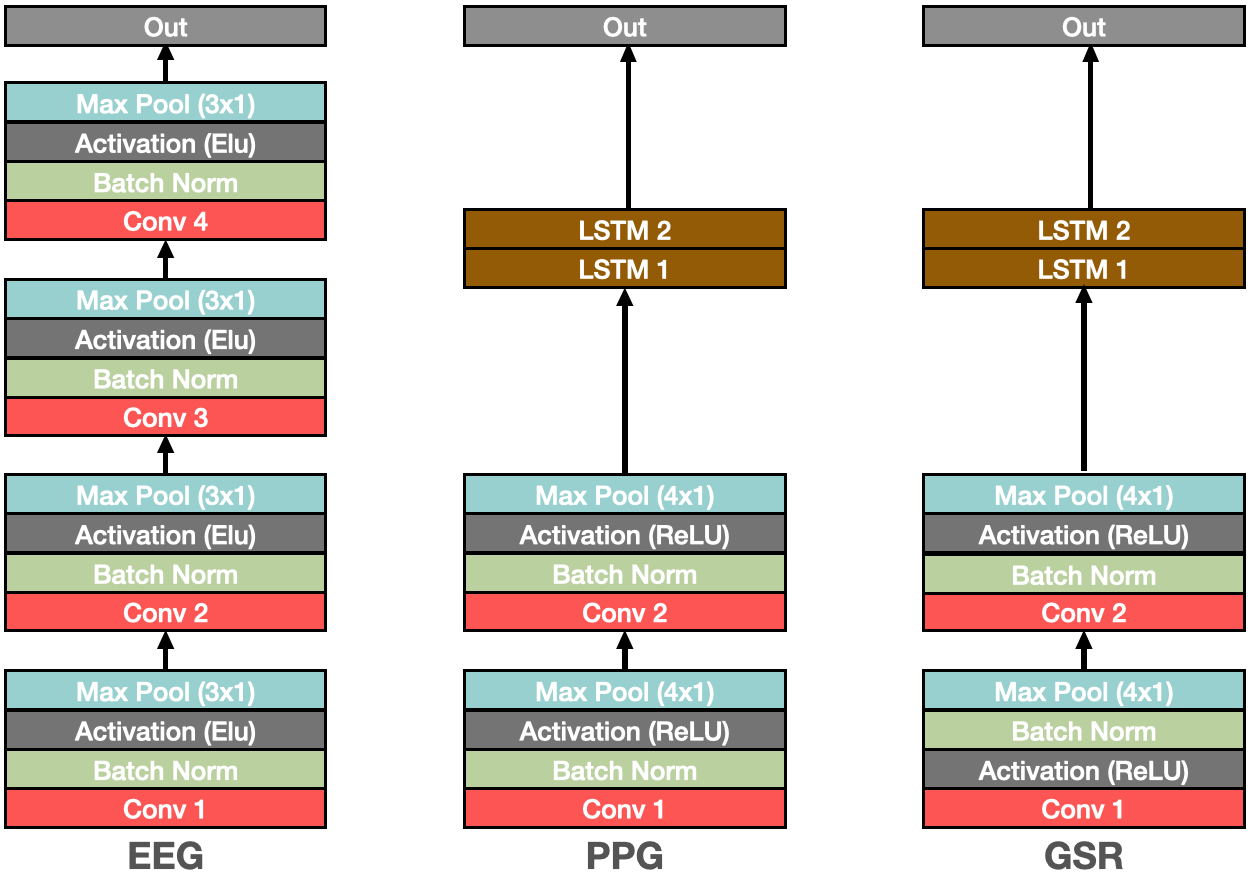
\includegraphics[scale=0.725]{single_model_architecture}
\label{fig:singlearchitecture}
\end{figure}

The utilized network for the EEG modality is a ConvNet, as proposed by \citeA{schirrmeister2017deep}. The network is designed to include four convolutional blocks, each constituting a convolutional layer, followed by a batch normalisation layer. The Exponential Linear Unit, hereafter referred to as "ELU", function is utilized as activation function, and is defined as equation \ref{eqn:elu}. Each convolutional block is closed with a max pooling layer of stride three.

\begin{equation}
\label{eqn:elu}
f(x)= 
\begin{Bmatrix}
x & x \geq0 \\ 
\alpha (e^x -1) & x<0
\end{Bmatrix}
\bigskip
\end{equation}

The utilized network for the GSR modality is a LSTM ConvNet network, inspired by the work of \citeA{sun2019hybrid} and  \citeA{dolmans2020perceived}. The network is designed to include two convolutional blocks, each constituting a convolutional layer, followed by a batch normalization layer, an activation layer and closed with a max-pooling layer of stride four. The Rectified Linear Unit, hereafter referred to as "ReLU", function is utilized as activation function, defined as equation \ref{eqn:relu}. Following these two convolutional blocks are two LTSM layers.

\begin{equation} 
\label{eqn:relu}
f(x)=max(0,x)
\bigskip
\end{equation}

Lastly, the utilized network for the PPG modality is inspired upon the network as proposed by \citeA{biswas2019cornet}. The nework opens with two convolutional blocks, each consisting of a convolutional layer, batch normalization layer, activation layer and closed with a max pooling layer of stride four. The utilized activation function is the ReLU, depicted as equation \ref{eqn:relu}. Following these convolutional blocks are two LTSM layers, equal to the GSR model. 

\subsubsection{Multi-modular Network: Architecture}
The network architecture that is utilized for the multi-modular approach is determined by a combination of the single-modular networks, as derived from the literature. The previously delineated design principles (i.e. the principles of modularity and generalizability) are taken into account when doing so. A visual representation of the multi-modular network is depicted as figure \ref{fig:multiarchitecture}.

\begin{figure}
\caption{Multi-modular Network Architecture}
\bigskip
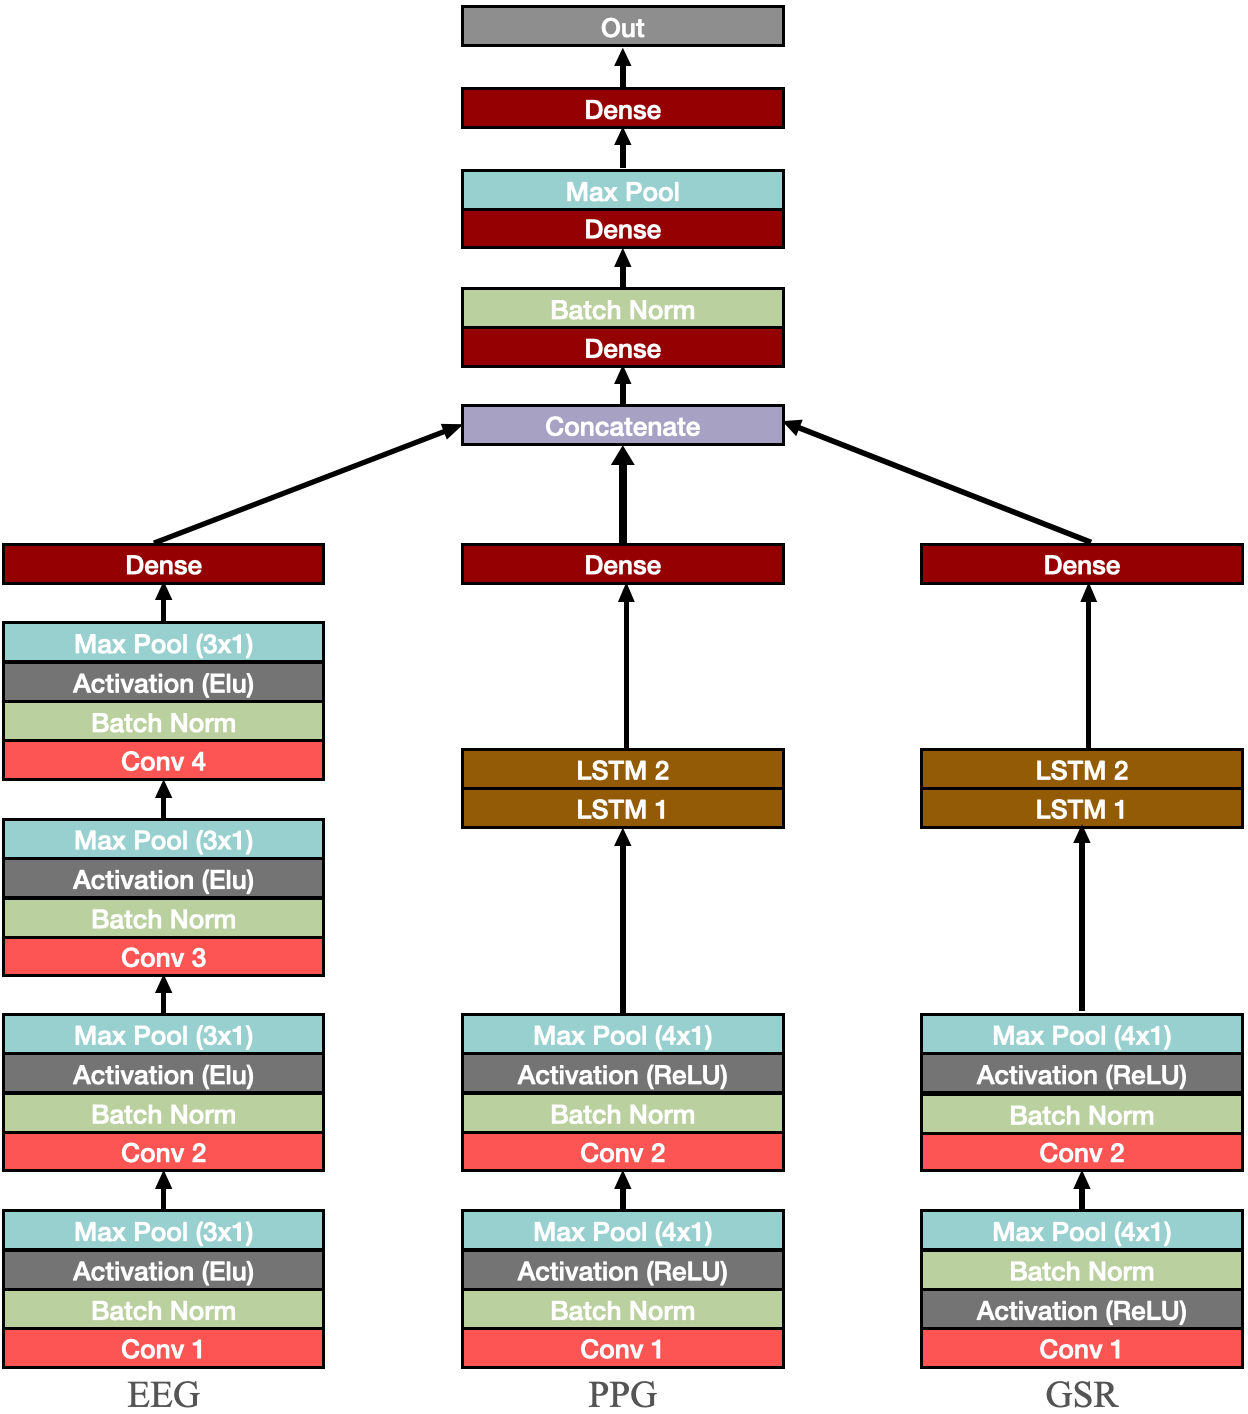
\includegraphics[scale=0.725]{multi_model_architecture}
\label{fig:multiarchitecture}
\end{figure}

In order to combine the previously delineated single-modular networks, each of these distinct parts are closed with one fully connected dense layer before feeding into the head network. This is done in order to flatten all inputs into a lower dimensional space, such that concatenation is possible. The head network consists of four dense layers. These layers are alternated with a batch normalization and max-pooling layer with the objective of stabilization. 

\subsubsection{Multi-modular Network: Variations}
Multi-modular classification in real-time by means of deep-learning requires an optimized network, as was elaborated upon in the introduction. Speed is a potential bottleneck, for a multi-modular network such as presented is substantially complex in nature. Therefore, several variations of the delineated network will be investigated upon, differing in their complexity. These variations are not made by changing the network architecture, whereas deviating from the proven network architecure is likely to be detrimental with regards to model performance. The aim is to propose a network that is fast enough for real-time classification, whilst maintaining the highest amount of accuracy as possible. Three different variations with regards to size of the network as depicted in figure \ref{fig:multiarchitecture} will therefore be considered.

Network size is understood as the amount of utilized filters for convolutional layers, and the amount of neurons for all other utilized layers. A decrease in the amount of filters and neurons constitutes a decrease in network size, and consequently a decrease in the amount of required calculations. This is likely to bring about an increase in speed. An overview of all three multi-modular network variations, and the amount of utilized neurons/filters is provided in table \ref{table:modelvariations}. Network 1 is referred to as the full network, and is the biggest in terms of size. The size of network 2 constitutes of 75 \% of the size of the full network. Network 3 constitutes of 50 \% of the size of the full network.

\bgroup
\def\arraystretch{1.6}%  
\begin{table}[h]
\centering
\caption{Model variation sizes}
\label{table:modelvariations}
\begin{tabular}{lllll}
\hline
        & EEG        & GSR        & PPG        & Head       \\ \hline
Network 1 & Conv1: 25  & Conv1: 128 & Conv1: 128 & Dense: 712 \\
        & Conv2: 50  & Conv2: 128 & Conv2: 128 & Dense: 356 \\
        & Conv3: 100 & LSTM1: 256 & LSTM1: 256 & Dense: 178 \\
        & Conv4: 200 & LSTM1: 256 & LSTM2: 256 &            \\ 
        \vspace{3ex}
        & Dense: 200 & Dense: 256 & Dense: 256 &            \\ \hline
Network 2 & Conv1: 18  & Conv1: 96  & Conv1: 96  & Dense: 534 \\
        & Conv2: 34  & Conv2: 96  & Conv2: 96  & Dense: 267 \\
        & Conv3: 75  & LSTM1: 192 & LSTM1: 192 & Dense: 134 \\
        & Conv4: 150 & LSTM1: 192 & LSTM1: 192 &            \\
        \vspace{3ex}
        & Dense: 150 & Dense: 192 & Dense: 192 &            \\ \hline
Network 3 & Conv1: 13  & Conv1: 64  & Conv1: 64  & Dense: 356 \\
        & Conv2: 25  & Conv2: 64  & Conv2: 64  & Dense: 178 \\
        & Conv3: 50  & LSTM1: 128 & LSTM1: 128 & Dense: 89  \\
        & Conv4: 100 & LSTM1: 128 & LSTM2: 128 &            \\
        & Dense: 100 & Dense: 128 & Dense: 128 &            \\ \hline
\end{tabular}
\vspace{2ex}

\begin{doublespacing}
{\raggedright \textit{Note:} For all convolutional layers the depicted number reflects the amount of utilized filters, whereas for LTSM layers it reflects the amount  of nodes. \par}
\end{doublespacing}
\end{table}
\egroup


\clearpage
\subsection{Model Evaluation}
The performance of the four network variations will be contrasted by means of several performance metrics. The utilized metrics constitute six well known and widely applied metrics, all constructed from the confusion matrix, depicted as table \ref{table:confusion}.

\bigskip
\bgroup
\def\arraystretch{1.6}%  
\begin{table}[h]
\centering
\caption{Confusion matrix}
\label{table:confusion}
\begin{tabular}{lll}
                                        & True Positive          & True Negative          \\ \cline{2-3} 
\multicolumn{1}{l|}{Predicted Positive} & \multicolumn{1}{l|}{a} & \multicolumn{1}{l|}{b} \\ \cline{2-3} 
\multicolumn{1}{l|}{Predicted Negative} & \multicolumn{1}{l|}{c} & \multicolumn{1}{l|}{d} \\ \cline{2-3} 
\end{tabular}
\end{table}
\egroup

The measures accuracy, sensitivity, specificity, PPV, NPV and F1 will be utilized in order to asses network performance. The network that performs best across these measures is considered to be the superior performing network. Table \ref{table:metrics} depicts the constitution of these performance metrics, by partly referring to confusion matrix depicted as table \ref{table:confusion}. 
\bigskip
\bgroup
\def\arraystretch{1.8}%  
\begin{table}[h]
\centering
\caption{Performance Metrics}
\label{table:metrics}
\begin{tabular}{ll}
\hline
Accuracy:                       & \(\frac{\!\!\!\!\!\!\!\!\!\!\!\!\!\!a+d}{a+b+c+d}\) \\
Sensitivity:                    & \(\frac{a}{a+c}\)                                   \\
Specificity:                    & \(\frac{d}{b+d}\)                                   \\
Positive Predicted Value (PPV): & \(\frac{a}{a+b}\)                                   \\
Negative Predicted Value:       & \(\frac{d}{c+d}\)                                   \\
F1-measure:                     & \(\frac{2*Sensitivity*PPV}{Sensitivity+PPV}\)       \\ \hline
\end{tabular}
\end{table}
\egroup

\newpage

\bibliographystyle{apacite}
\bibliography{References}

\end{document}
